\subsection{Feature Extraction}
As demonstrated by \cite{Raza_Mehmood_Ullah_Ahmad_Choi_On_2019} and \cite{Chen_Sun_Chen_Xie_Wu_Xu_2021}, MFCCs
are highly effective features for heartbeat classification. In addition to MFCCs,
we incorporated other features to capture various characteristics of heart sounds, enhancing the classification accuracy.
The features used are explained in the following section.

\subsubsection*{Features Type}  % Andrea
\textbf{MFCC}\newline
Mel-Frequency Cepstral Coefficients (MFCCs) are representations of the short-term power spectrum of sound.
They are derived by taking the Fourier transform of a signal, mapping the powers of the spectrum onto the mel
scale, taking the logarithm, and then performing a discrete cosine transform. MFCCs are effective in capturing
the timbral texture of audio and are widely used in speech and audio processing due to
their ability to represent the envelope of the time power spectrum.
In heartbeat classification, MFFCs can reflect the different perceived quality of heart sounds,
such as the presence of murmurs or other anomalies.

\vspace{0.3cm}\noindent
\textbf{Chroma STFT}\newline
Chroma features represent the 12 different pitch classes of music.
They are particularly useful for capturing harmonic and melodic characteristics in music.
By mapping audio signals onto the chroma scale, these features can identify pitches regardless
of the octave, making them useful for analyzing harmonic content in heart sounds.

\vspace{0.3cm}\noindent
\textbf{RMS}\newline
Root Mean Square (RMS) measures the magnitude of varying quantities, in this case,
the amplitude of an audio signal. It is a straightforward way to compute the energy of
the signal over a given time frame. RMS is useful in audio analysis for detecting volume
changes and can help identify different types of heartbeats based on their energy levels.
For example, in a given timeframe the RMS may be altered by the presence of a murmur
with respect to a normal heart sound.

\vspace{0.3cm}\noindent
\textbf{ZCR}\newline
Zero-Crossing Rate (ZCR) is the rate at which a signal changes sign, indicating how often the signal
crosses the zero amplitude line. It is particularly useful for detecting the noisiness and the temporal
structure of the signal. In heartbeat classification, ZCR can help differentiate between normal and abnormal
sounds by highlighting changes in signal periodicity.

\vspace{0.3cm}\noindent
\textbf{CQT}\newline
Constant-Q Transform (CQT) is a time-frequency representation with a logarithmic frequency scale, making it
suitable for musical applications. Since it captures more detail at lower frequencies, it may be useful for analyzing
the low-frequency components of heart sounds.

\vspace{0.3cm}\noindent
\textbf{Spectral Centroid}\newline
The spectral centroid indicates the center of mass of the spectrum and is often perceived as the brightness of a
sound. It is calculated as the weighted mean of the frequencies present in the signal, with their magnitudes as
weights. In heart sound analysis, a higher spectral centroid can indicate sharper, more pronounced sounds,
while a lower centroid suggests smoother sounds.

\vspace{0.3cm}\noindent
\textbf{Spectral Bandwidth}\newline
Spectral bandwidth measures the width of the spectrum around the centroid, providing an indication of the range
of frequencies present. It is calculated as the square root of the variance of the spectrum. This feature helps
in understanding the spread of the frequency components in the heart sounds, which can be indicative of different
heart conditions.

\vspace{0.3cm}\noindent
\textbf{Spectral Roll-off}
Spectral roll-off is the frequency below which a certain percentage of the total spectral energy lies. It is
typically set at 85\% and helps distinguish between harmonic and non-harmonic content. In heartbeat classification,
spectral roll-off can be used to differentiate between sounds with a concentrated energy distribution and those with more dispersed energy.
\subsubsection*{Sampling Rate Selection} % Andrea
\label{sec:sampling_rate}
The sampling rate of the data were heterogeneous, ranging from 4000 Hz to 44100 Hz, with a majority of the data being sampled at 4000 Hz.
To assess the impact of the sampling rate on the classification performance, we trained different models on
different features, extracted at different sampling rates and from various intervals. Each model is then
evaluated using different metrics, taking into account the class imbalance issue.
We also considered a possible dependency between the sampling rate and the extraction interval, as shown
in Algorithm \ref{alg:sr_choice}.

\begin{algorithm}
    \small
    \caption{Sampling rate and Interval choice}
    \label{alg:sr_choice}
    \begin{algorithmic}[1]
        \State \textbf{Input:}
        \State {features} = [\texttt{mfcc30 \& 120}, \texttt{cqt30 \& 70}, \texttt{chroma12}]
        \State {sampling\_rates} = [\texttt{mix}, \texttt{4000}]
        \State {extraction\_intervals} = [\texttt{0.5}, \texttt{1}, \texttt{2}, \texttt{3}]
        \State {models} = [\texttt{rf}, \texttt{svm-rbf}, \texttt{lr}]
        \State {metrics} = [\texttt{macrof1}, \texttt{mcc}]

        \vspace{0.2cm}
        \For{sr \textbf{in} sampling\_rates}
        \For{interval \textbf{in} extraction\_intervals}
        \For{feature \textbf{in} features}
        \State \textbf{extract} {feature} with {interval} at {sr}
        \For{model \textbf{in} models}
        \State \textbf{train} {model} with extracted {feature}
        \For{metric \textbf{in} metrics}
        \State \textbf{evaluate} {model} with {metric}
        \EndFor
        \EndFor
        \EndFor
        \EndFor
        \EndFor

        \State \textbf{Output:}
        \State Given all the results, group by \texttt{model} and average the values of a specific \texttt{metric} across \texttt{features} and \texttt{intervals}

    \end{algorithmic}
\end{algorithm}

\noindent
The results, reported in Figure \ref{fig:FE_sampling_rate.png} showed no evident advantage to using a mix of sampling frequencies over a fixed resampled sample rate.
Moreover, employing a fixed sample rate of 4000 Hz reduces the risk of introducing bias, enhances efficiency,
and permits the use of a broader range of features and models.

\begin{figure}[H]
    \centering
    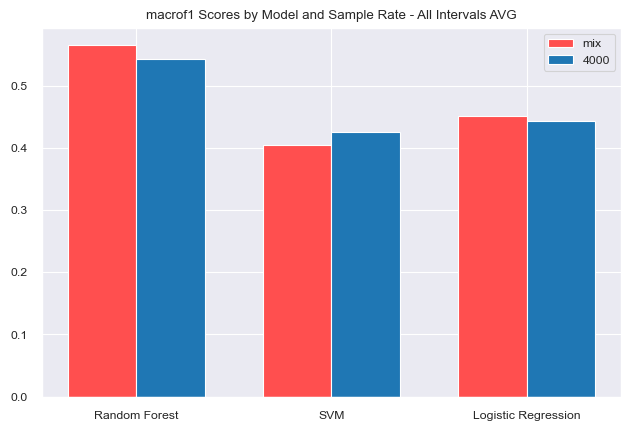
\includegraphics[width=1\columnwidth]{./images/FE_sampling_rate.png}
    \caption{Comparison of the macro F1 score for different sampling rates.}
    \label{fig:FE_sampling_rate.png}
\end{figure}


\subsubsection*{Extraction Interval Selection}  % Andrea
\label{sec:extraction_interval}
The extraction interval refers to the duration of the audio segment from which the features are extracted.
Using algorithm \ref{alg:sr_choice}, we evaluated the performance of 0.5, 1, 2, and 3-second intervals
on the classification task. It is important to note that the interval choice affects the number of samples
available for training and evaluation, so in case of a limited number of samples, this choice should no be based
solely on the performance of the model. The results, showed that a 2-second interval yielded the best performance,
however it also reduced the number of samples, impeding a correct training and evaluation of the models.
As a consequence, we picked a 1-second interval as a compromise.

\subsubsection*{Number of Features per Type} % Davide
Now the focus is on identifying the optimal number of features for different types of audio features (MFCC, Chroma, CQT, etc.).
Each type of feature can consist of a varying number of individual features, and it is crucial to determine the optimal number to maximize
the model's performance. Proper feature selection is vital because it directly impacts the efficiency, accuracy,
and generalizability of the machine learning model. Including too many features can lead to overfitting, increased computational costs,
and degraded performance due to the curse of dimensionality. On the other hand, using too few features can result in underfitting,
where the model fails to capture the necessary patterns in the data. Therefore, the goal of this study is to identify the optimal number of features
for each type to ensure the model is both robust and efficient.

\paragraph{Determining the Optimal Number of Features}

To maximize the model's performance, it is crucial to determine the optimal number of features for each type.
This was achieved using a `One Model per Feature' approach, which involved the following steps:

\begin{algorithm}
    \caption{Feature Optimization Process}
    \begin{algorithmic}[1]
        \State \textbf{Step 1:} Extract feature sets with varying sizes: 12, 20, 30, 40, 60, 70, 90, and 120 features for each type.
        \State \textbf{Step 2:} For each feature set, train three classifiers: SVM, Random Forest,
        and Logistic Regression.
        \State \textbf{Step 3:} Evaluate the performance of each model.
    \end{algorithmic}
\end{algorithm}

\begin{figure*}[htbp]
    \centering
    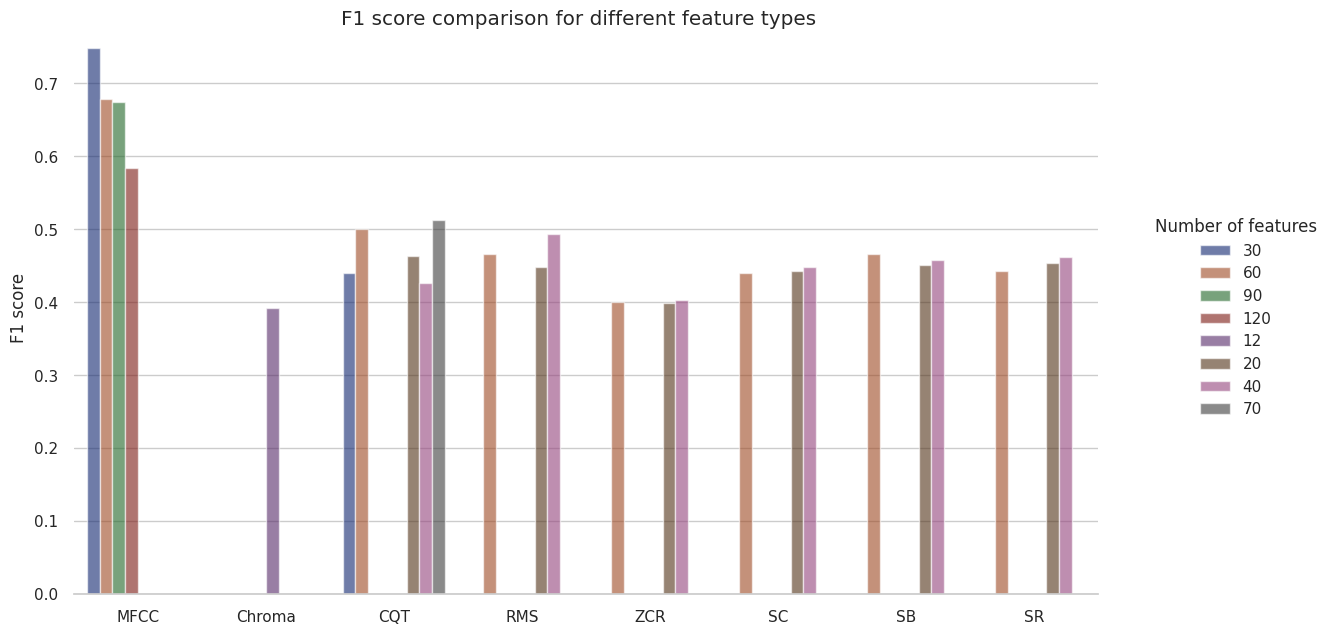
\includegraphics[width=\textwidth]{../images/n_feature_per_type.png}
    \caption{F1 score per number of features}
    \label{fig:n_feature_per_type}
\end{figure*}

\noindent
Figure \ref{fig:n_feature_per_type} shows the results obtained for each type of feature with the Random Forest model,
which significantly outperformed the other classifiers.
From the figure, we can observe the following trends for each feature type:
\begin{itemize}
    \item \textbf{MFCC:} The MFCC features consistently achieved the highest F1 scores, peaking around 0.7.
          This indicates their effectiveness for the classification task. Interestingly, the number of MFCC features (ranging from 30 to 120)
          did not drastically affect performance, suggesting that even a smaller set of MFCC features can be highly informative.
    \item \textbf{CQT:} The CQT features showed moderate performance, with F1 scores around 0.4 to 0.5. The optimal number of features was around 70,
          beyond which there was no significant improvement.
    \item \textbf{RMS:} RMS features exhibited F1 scores ranging from 0.4 to 0.5, with optimal performance achieved with around 70 features.
    \item \textbf{ZCR, Spectral Centroid (SC), Spectral Bandwidth (SB), and Spectral Roll-off (SR):}
          The F1 scores for these features generally stabilized around 0.4 to 0.5.
          Increasing the number of features beyond 40 did not result in significant performance gains and could even degrade the model's performance.
          This suggests that adding too many features, especially those without strong predictive power, can confuse the model and degrade its performance.
\end{itemize}
\paragraph{Optimal Number of Features}

Based on the results, the optimal number of features for each type is shown in Table \ref{tab:optimal_features}.
\rowcolors{2}{blue!8}{blue!18}
\begin{table}[h]
    \centering
    \small
    \begin{tabular}{|lc|}
        \hline
        \textbf{Feature Type} & \textbf{Optimal Number of Features} \\
        \hline
        MFCC                  & 30                                  \\
        Chroma                & 12                                  \\
        CQT                   & 70                                  \\
        RMS                   & 40                                  \\
        ZCR                   & 40                                  \\
        Spectral Centroid     & 40                                  \\
        Spectral Bandwidth    & 60                                  \\
        Spectral Roll-off     & 40                                  \\
        \hline
    \end{tabular}
    \caption{Optimal number of features for each type}
    \label{tab:optimal_features}
\end{table}